\chapter{Computer Architecture}
\graphicspath{ {./images/} }


Computer architecture in layman terms is all about building a computer machine with some or total specification and detailing of how a set of software and hardware technologies interact with each other as to form a computer system.It refers to how a computer system is designed and what technologies it is compatible with.\\

One of the most followed Logical model of computer architecture is \textbf{Von Neumann's Architecture}. This was proposed by the mathematician \textit{John von Neumann} in 1945. It describes the design of an electronic computer with its CPU, which includes the arithmetic logic unit, control unit, registers, memory for data and instructions, an input/output interface and external storage functions. It follows that an instruction fetch and data operation cannot be performed at the same time. Another used architecture is \textbf{Harvard's Architecture} which is also similar to Neuman's Architecture except that \underline{it uses different physical paths or data buses for carrying data and instruction}. This idea has lead to creation of parallelism and this distinction has evolved over to reason for the different Cache mechanisms used for a \textit{Random Accessed Memory (RAM)} and \textit{Read Write Memory (RWM)} type memory storage.\\

Let's now look at the basic parts of computer architecture.\\   

% Inserting Images in a arow

\begin{figure}[!htb]
\minipage{0.4\textwidth}
  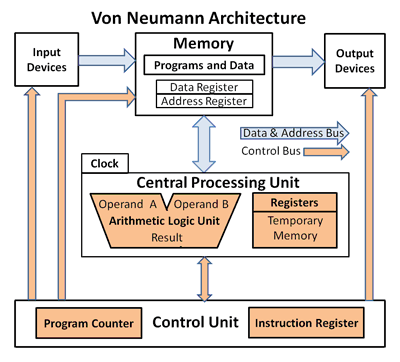
\includegraphics[width=\linewidth]{von_neuman}
  %\caption{A really Awesome Image}\label{fig:awesome_image1}
\endminipage\hfill
\minipage{0.4\textwidth}
  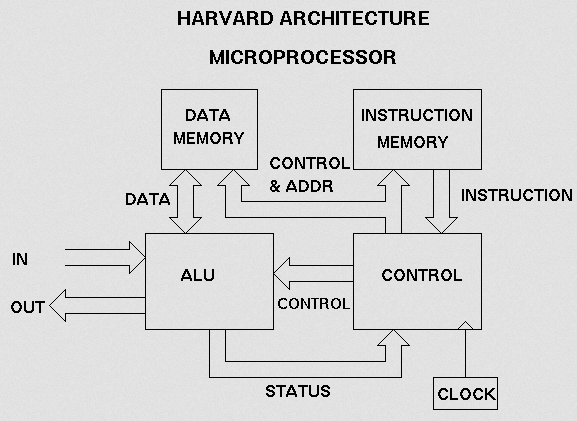
\includegraphics[width=\linewidth]{harvard_arch}
  %\caption{A really Awesome Image}\label{fig:awesome_image2}
\endminipage\hfill
% \minipage{0.32\textwidth}%
%   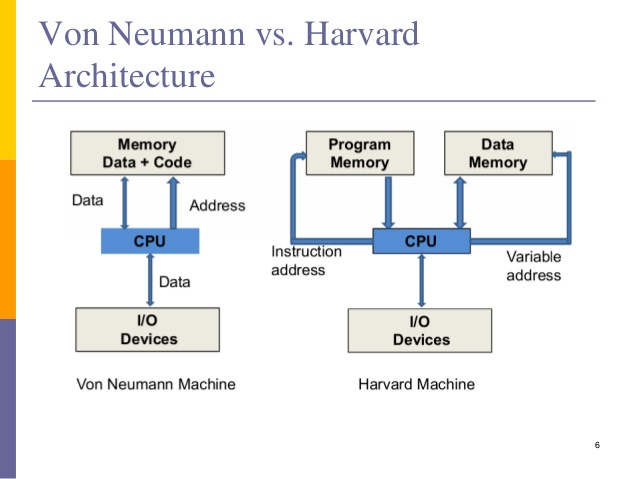
\includegraphics[width=\linewidth]{difference}
%   \caption{A really Awesome Image}\label{fig:awesome_image3}
% \endminipage
\end{figure}


\section{Instruction Set Architecture}
Instruction Set Architecture (ISA) serves as the interface between computer software and hardware. It is a set of rules or instructions that define the working of a computer. These have evolved overtime due to numerous optimizations implemented for the same hardware. Such improvements have led to more abstractness. For example, most of present ISA deal with pointers rather than directly referring to registers in the machine byte code implementation. ISA define some of the very fundamental data types that correspond to some fixed bit size storage in memory. It handles very low-level control flow and Logic operations. Its very important to understand many compiler-implementations can produce same Instruction Set. Instruction Set is defined only for a hardware and assembly-level machine codes should follow these IS specifications only. \\

An ISA may be classified by their implementation complexity. A \textbf{Complex Instruction Set Computer (CISC)} has many special instructions but can be realized with other basic instructions too thus a \textbf{Reduced Instruction Set Computer (RISC)} is used that increases efficiency by implementing only those instructions that are frequently used in programs, and also some special instructions if required and made possible by an \underline{appropriate memory-time tradeoff}.\\ 


Other types include \textbf{Very Long Instruction Word} (VLIW) architectures, and the closely related \textbf{Long Instruction Word (LIW)} and \textbf{Explicitly Parallel Instruction Computing} (EPIC) architectures. These architectures seek to exploit instruction-level parallelism with less hardware than RISC and CISC by making the compiler responsible for instruction issue and scheduling.\\

\section{Microarchitecture Design}

Microarchitecture design also called computer organization desing deals with the ways a given instruction set architecture (ISA), is implemented in a particular processor. The microarchitecture is usually represented as diagrams that describe the interconnections of the various microarchitectural electronic hardware elements of the machine which includes components from basic registers to complete ALU. These diagrams generally separate the datapath and instruction control path. Some important terms related to the microarchitecture design are given here under.\\

The \textbf{Instruction Cycle} is the basic operational process of a computer system. It is the process by which a computer retrieves a program instruction from its memory, determines what actions the instruction describes, and then carries out those actions. \textbf{Instruction Pipelining} is a technique for implementing instruction-level parallelism within a single processor. \textbf{Cache} is simply very fast memory. It can be accessed in a few cycles as opposed to many-step access or other type of memory. \textbf{Multiprocessing} is the use of two or more central processing units (CPUs) within a single computer system. The term also refers to the ability of a system to support more than one processor or the ability to allocate tasks between them. \textbf{Multithreading} or \textbf{Concurrency} is the ability of a central processing unit (CPU) (or a single core in a multi-core processor) to execute multiple processes or threads concurrently, supported by the operating system. \\ 

\section{Logic Synthesis and Implementation}

Finally when both the ISA and Microarchitecture design are available, the next thing to do is finally implement it.This includes all the logic implementation (the gate logic), Circuit Implementation and desingn validation through FPGAs. The way it works is making complete circuitary on a FPGA board and then performing error reductions to improve efficiency. Else one may simulate the proposed $\mu$-architecture on an existing machine or computer system.\\


Here comes the intersting part that follows from the \underline{\textbf{Church-Turing Hypothesis}} that says any first order recursive and computable function can be well simulated in a \textbf{Turing-Complete machine}. All classical machines are however not perfectly turing complete and some functions can't be simulated on them. Here on \textbf{Destusch} added his hypothesis claming the \textit{Quantum Parallelism} couldn't be sufficiently simulated because of much large randomness in the resluting values.
